%%% Prepared by Wai Qian Tham, on 4 June 2024. 
%% Prepared with comments and instructions for report writing. However, the writing guide is specifically for scientific writing, following IEEE guidelines. Do consult library services or any departmental writing guidelines for report writing. 
%% This main page contains the preamble, and the only content here is the title and the abstract. Other content writing can be done in the .tex files in the other folders. 

\documentclass[a4paper]{article} 
% \documentclass[a4paper, twocolumn]{article}

%% Language and font encodings
\usepackage[english]{babel}
\usepackage[utf8]{inputenc}
\usepackage[T1]{fontenc}
%% Sets page size and margins
\usepackage[a4paper,top=2cm,bottom=2cm,left=2.5cm,right=2.5cm,marginparwidth=1.75cm]{geometry}


%% Useful packages
\usepackage{float} % Para usar [H] en figuras
\usepackage{subcaption}
\usepackage{caption}
\usepackage{amsmath}
\usepackage{graphicx}
\usepackage{tabularx}
\usepackage{xcolor}
\definecolor{tcdBlue}{RGB}{5, 105, 185}
\usepackage[colorlinks=true,allcolors=.,urlcolor=blue]{hyperref} % allowing hyperlinking of references. You can set the colour of the links or turn the colorlinks to false if no colour preferable. 
\usepackage[numbers]{natbib} % for Vancouver numbering style citation. Remove the [numbers] command for author-year Harvard style referencing. 


%% optional changes to the style. Comment (Ctrl+/) to remove these options. 
% change font to sans-serif fonts. 
\renewcommand{\familydefault}{\sfdefault}
% Format chapter headings appropriately to include tcd blue. 
\usepackage{titlesec}
\titleformat{\section}[hang]{\normalfont\Large\bfseries\color{tcdBlue}}{\thesection}{1em}{}{}


%% For nomenclature. Comment away if not used. 
% \usepackage{nomencl} % for nomenclature
% \usepackage{etoolbox} % to group nomenclature
% \usepackage{multicol} % for multiple columns in a page/table

\hyphenation{op-tical net-works semi-conduc-tor}

\begin{document}
\title{Optimización del Problema del Viajante mediante Algoritmos Genéticos: Comparación de Métodos de Selección y Inicialización}
\author{Silupú Peñaranda Rodrigo}
\maketitle

\begin{abstract}
El Problema del Viajante (TSP) es un desafío clásico en la optimización combinatoria, donde se busca la ruta más corta que permita visitar todas las ciudades una vez y regresar al punto de partida. Este trabajo detalla la implementación de un GA para resolver el TSP. La implementación incluye inicialización de la población, cálculo de aptitud, selección, cruce y mutación, y la ejecución del algoritmo a lo largo de múltiples generaciones. Se comparan métodos de selección como ruleta, rango y torneo, encontrando que el método de torneo ofrece un mejor rendimiento en términos de optimización de rutas. Esta investigación demuestra la eficacia de los GA en la resolución de problemas complejos de optimización.
\end{abstract}


% \tableofcontents % Optional. Remove if unnecessary (or ugly). 
% % to add to nomenclature, input:
% \nomenclature{P*}{\varepsilon}{Efficiency}
% *the subgroup of the nomenclature, in this instant, P for physical constant (Ctrl+F search \nomgroup)
\makenomenclature
\renewcommand\nomgroup[1]{%
  \item[\bfseries
  \ifstrequal{#1}{P}{\large Physical Constants}{%
  \ifstrequal{#1}{C}{\large Chemical Symbols}{%
  \ifstrequal{#1}{S}{\large Other Symbols}{%
  \ifstrequal{#1}{A}{\large Abbreviations}{}}}}%
]}

\setlength{\nomitemsep}{-\parskip} % Baseline skip between items
% to set double columns for nomenclature. Comment out if single column preferred. 
\renewcommand*\nompreamble{\begin{multicols}{2}}
\renewcommand*\nompostamble{\end{multicols}}

\hline
\printnomenclature
\hline
\vspace{1ex} % Optional. Remove if unnecessary. 
\section{Introducción}

En el ámbito de la optimización y búsqueda de soluciones, los algoritmos genéticos han demostrado ser herramientas efectivas debido a su capacidad para explorar vastos espacios de solución y encontrar óptimos globales. Estos algoritmos se inspiran en los principios de la evolución natural y utilizan mecanismos como la selección, cruce y mutación para generar nuevas soluciones a partir de las existentes.

\vspace{1em} 
El presente trabajo se enfoca en la implementación y comparación de diferentes métodos de selección y inicialización de población en algoritmos genéticos aplicados a un problema de optimización de rutas en un conjunto de 100 ciudades. En particular, se llevarán a cabo dos experimentos principales:

\begin{itemize}
\item Experimento 1: Implementación y comparación de la solución obtenida usando los métodos de selección: {\it Roulette wheel selection}, {\it Rank-based selection}, {\it Fitness scaling} y {\it Tournament selection}.
\item Experimento 2: Implementación y comparación de la solución obtenida usando los métodos de inicialización de población: {\it random}, {\it heuristic} y {\it hybrid initialization}.
\end{itemize}

Para cada experimento, se guardarán los valores de aptitud en intervalos específicos de generaciones y se generarán gráficos que mostrarán cómo cada método afecta la búsqueda de soluciones. 

 % introduction to the report. 
\section{Implementación}

En esta sección se detallará la implementación del código, el cual puede encontrarse en el siguiente \href{https://github.com/rodrigosilupu/TSP-GeneticAlgorithm-Optimization}{enlace}.

El Problema del Viajante (TSP) es un problema clásico en el campo de la optimización combinatoria, donde el objetivo es encontrar la ruta más corta que permita a un viajante visitar todas las ciudades exactamente una vez y regresar al punto de partida. Este problema es NP-difícil, lo que lo hace un candidato ideal para ser abordado mediante Algoritmos Genéticos (GA).

La implementación del GA para el TSP se basa en la clase  \textbf{'GeneticAlgorithmTSP'}, que encapsula los componentes principales del algoritmo. Esta clase se inicializa con una lista de ciudades, el tamaño de la población, el número de generaciones, la tasa de mutación, el método de selección y el método de inicialización de la población. Los componentes del algoritmo son los siguientes:

\begin{itemize}
\item Inicialización de la Población: La función \textbf{'initialize\_population'} genera la población inicial. En el primer experimento, cada individuo se crea mediante permutaciones aleatorias de las ciudades. En el segundo experimento, se introducen métodos de inicialización adicionales: aleatoria (random), heurística (heuristic) y una combinación de ambas (hybrid).
\item Cálculo de Aptitud: La función \textbf{'fitness'} calcula la distancia total de un recorrido, sumando las distancias euclidianas entre ciudades consecutivas y cerrando el ciclo al regresar a la ciudad de origen.
\item Selección: La función \textbf{'select'} elige a los padres para la generación siguiente. Se implementan métodos de selección como la ruleta, el rango y el torneo, con el torneo siendo el método utilizado en el segundo experimento.
\item Cruce y Mutación: El método \textbf{'crossover'} combina partes de dos padres para generar un nuevo individuo, mientras que la función mutate introduce variaciones aleatorias en los individuos para mantener la diversidad genética.
\item Ejecución del Algoritmo: El método \textbf{'run'} ejecuta el GA a lo largo de múltiples generaciones. En cada generación, se evalúan las aptitudes de los individuos, se seleccionan padres, se generan nuevos individuos mediante cruce y mutación, y se registra la mejor aptitud alcanzada.
\end{itemize}
 % background of article or theory



\section{Resultados}


\subsection{Experimento 1: Comparación de Métodos de Selección}
En el primer experimento, se comparan tres métodos de selección: ruleta, rango y torneo. Cada método se evalúa utilizando una población de 100 individuos, a lo largo de 3000 generaciones y con una tasa de mutación del 1\%. La función \textbf{'plot\_fitness'} grafica la evolución de la aptitud a lo largo de las generaciones, permitiendo comparar visualmente el desempeño de cada método. Además, la función \textbf{'plot\_route'} muestra la mejor ruta encontrada por cada método.

La siguiente gráfica muestra la evolución de la aptitud a lo largo de las generaciones para cada método de selección:

\begin{figure}[H]
  \centering
  \caption{Comparación de la evolución de la aptitud para los métodos Ruleta, Rango y Torneo}
  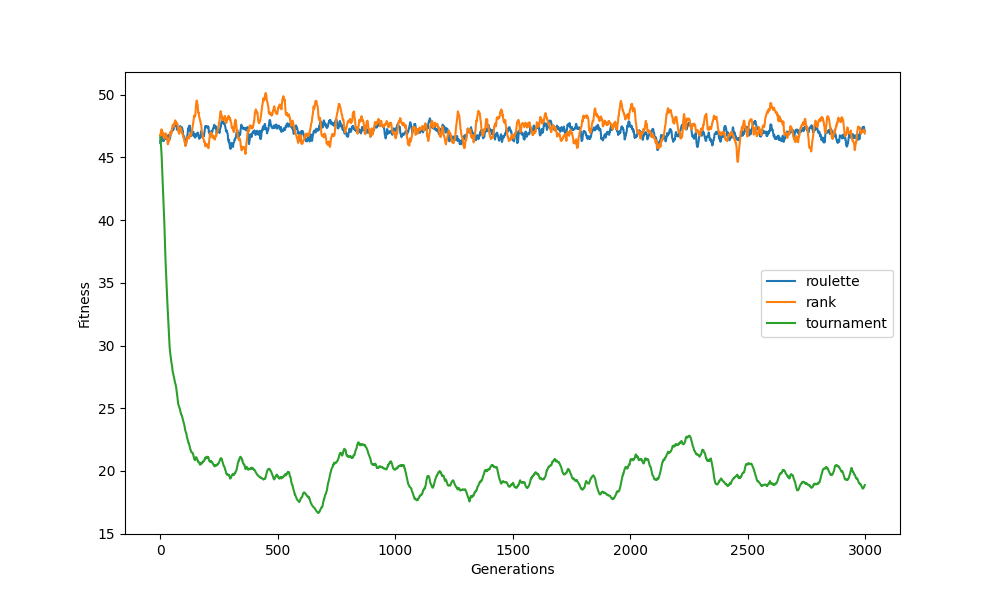
\includegraphics[width=0.8\linewidth]{3_method/Graphs/fitness_comparison_experimento1.png}
\end{figure}

Las mejores rutas encontradas por cada método son las siguientes:

\begin{figure}[H]
  \centering
  \caption{Mejores rutas encontradas por los métodos Ruleta, Rango y Torneo}
  \begin{minipage}{0.32\textwidth}
    \centering
    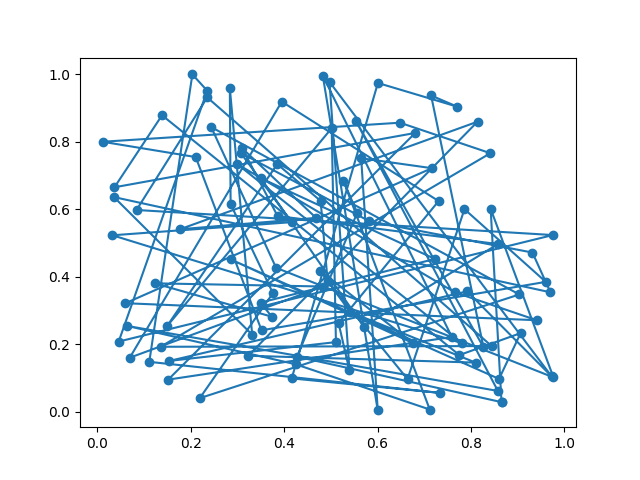
\includegraphics[width=\linewidth]{3_method/Graphs/best_route_(roulette).png}
    \subcaption{Mejor ruta para el método Ruleta}
  \end{minipage}\hfill
  \begin{minipage}{0.32\textwidth}
    \centering
    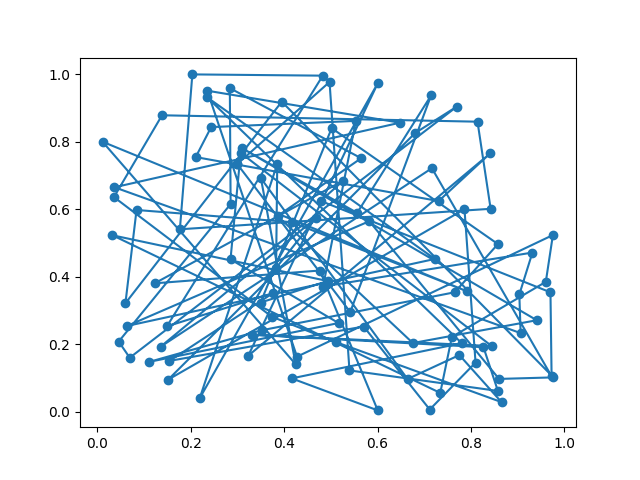
\includegraphics[width=\linewidth]{3_method/Graphs/best_route_(rank).png}
    \subcaption{Mejor ruta para el método Rango}
  \end{minipage}\hfill
  \begin{minipage}{0.32\textwidth}
    \centering
    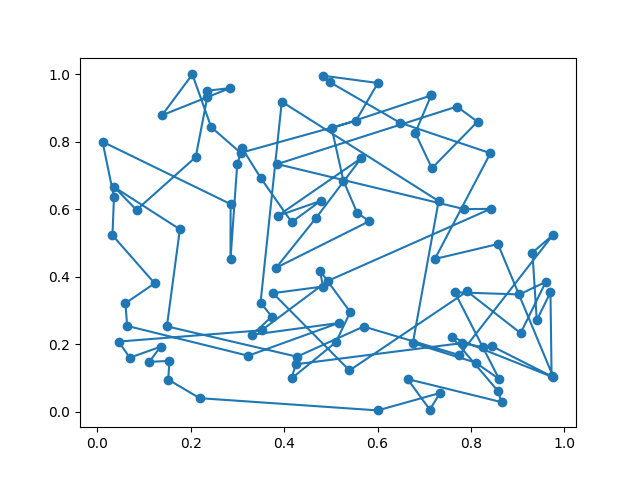
\includegraphics[width=\linewidth]{3_method/Graphs/best_route_(tournament).png}
    \subcaption{Mejor ruta para el método Torneo}
  \end{minipage}
\end{figure}


\subsection{Experimento 2: Comparación de Métodos de Inicialización} 
En el segundo experimento, se comparan tres métodos de inicialización de la población: aleatoria, heurística y una combinación híbrida de ambos. Se utiliza una población de 100 individuos, una tasa de mutación del 1\% y se ejecuta el algoritmo durante 3000 generaciones con selección por torneo. El método de inicialización heurística introduce un componente de conocimiento previo en la generación de los individuos, mientras que el método híbrido busca combinar los beneficios de la aleatoriedad y la heurística. 

La siguiente gráfica muestra la evolución de la aptitud a lo largo de las generaciones para cada método de inicialización:

\begin{figure}[H]
  \centering
  \caption{Comparación de la evolución de la aptitud para los métodos de inicialización Aleatorio, Heurístico e Híbrido}
  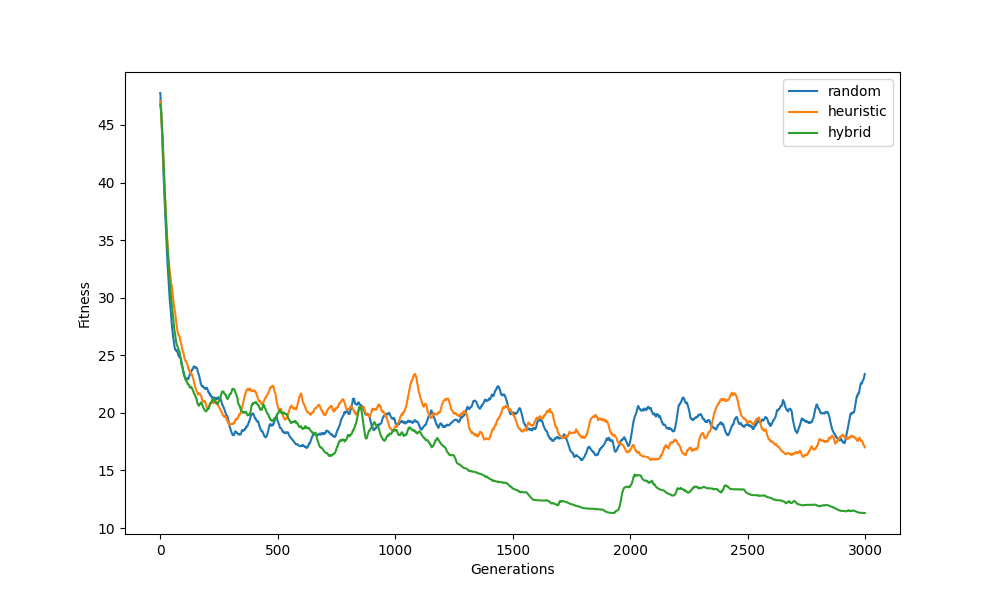
\includegraphics[width=0.8\linewidth]{3_method/Graphs/fitness_comparison_experimento2.png}
\end{figure}

Las mejores rutas encontradas por cada método son las siguientes:


\begin{figure}[H]
  \centering
  \caption{Mejores rutas encontradas por los métodos Aleatorio, Heurístico y Híbrido}
  \begin{minipage}{0.32\textwidth}
    \centering
    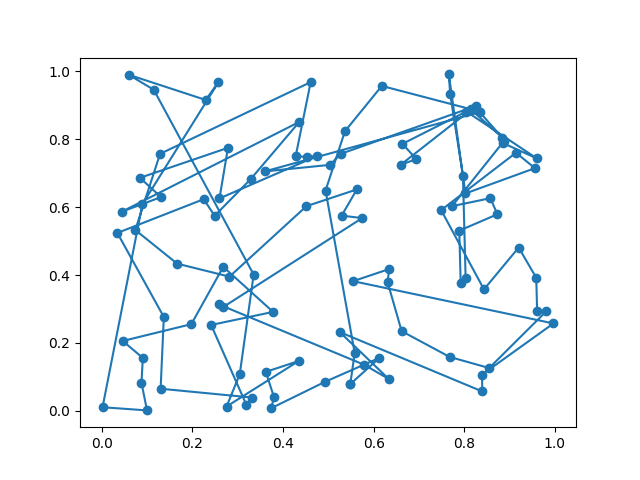
\includegraphics[width=\linewidth]{3_method/Graphs/best_route_(random).png}
    \subcaption{Mejor ruta para el método Aleatorio}
  \end{minipage}\hfill
  \begin{minipage}{0.32\textwidth}
    \centering
    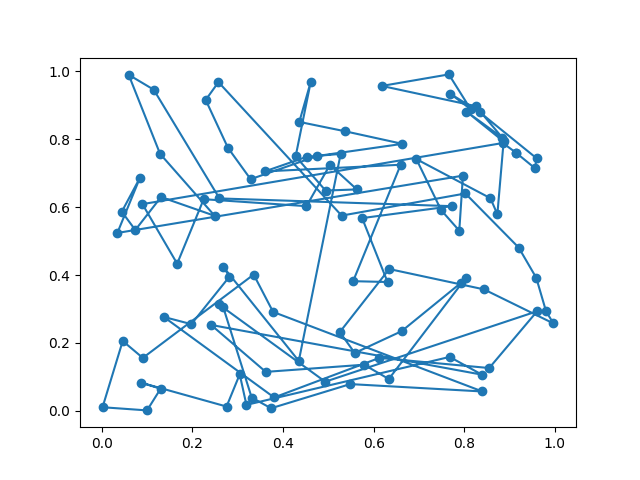
\includegraphics[width=\linewidth]{3_method/Graphs/best_route_(heuristic).png}
    \subcaption{Mejor ruta para el método Heurístico}
  \end{minipage}\hfill
  \begin{minipage}{0.32\textwidth}
    \centering
    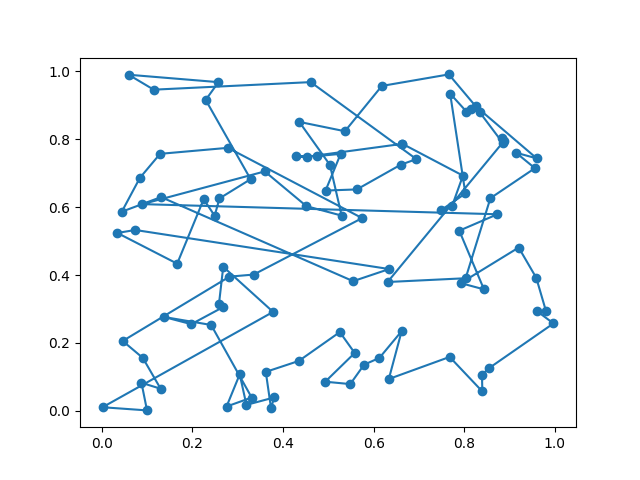
\includegraphics[width=\linewidth]{3_method/Graphs/best_route_(hybrid).png}
    \subcaption{Mejor ruta para el método Híbrido}
  \end{minipage}
\end{figure}
 % methodology
\section{Discusión}
A continuación, se presenta un análisis detallado de ambos experimentos, destacando las características y el desempeño de cada método.

\subsection{Experimento 1: Comparación de Métodos de Selección}

A comparación de los modelos ruleta y rango, el método torneo presenta una convergencia más rápida y alcanza una aptitud final más baja en comparación con los métodos de ruleta y rango. Esto puede deberse a que los métodos de selección por ruleta y rango, aunque efectivos en ciertos contextos, pueden ser más susceptibles a problemas de diversidad y fluctuaciones en la aptitud. Por otro lado, el método de torneo, selecciona un subconjunto aleatorio (en este caso, de tamaño 5) y elige el individuo con la mejor aptitud dentro de ese subconjunto. Esto proporciona una presión selectiva controlada, ya que solo los mejores individuos dentro de cada subconjunto tienen la oportunidad de ser seleccionados. 


\subsection{Experimento 2: Comparación de Métodos de Inicialización}

Se observa que el método híbrido logra la aptitud más baja, seguido por el heurístico y finalmente el aleatorio.Esto puede deberse a que el método híbrido combina la diversidad introducida por la aleatoriedad con la dirección proporcionada por las heurísticas. En este sentido, el método híbrido puede explotar de manera más efectiva el espacio de búsqueda, logrando una convergencia eficiente y robusta. % elaborating on the results
\addcontentsline{toc}{section}{Acknowledgements}

 
%% References
% \\bibliographystyle{unsrtnat} % Vancouver reference style (numbering). 
% \bibliographystyle{agsm} % Harvard reference style (author-year). 
% \\bibliography{B_bibs/bibliography}
% \\addcontentsline{toc}{section}{Bibliography}

\end{document}